\section[Collaborative filtering]{Collaborative filtering}
\begin{frame}
	\frametitle{Collaborative filtering}
	
    \hspace{-1cm}
	\begin{minipage}{0.7\linewidth}
    \begin{itemize}\itemsep1em
		\item Method of making automatic predictions (filtering) about the interests of a user by collecting preferences or taste information from many users. It is provided.
		\item 2 types filtering:
		\fontsize{10}{14}\selectfont
		\begin{itemize}
    	  \item \textbf{User-based filtering}
    	  \item \textbf{Item-based filtering}
    	 \end{itemize}
    	 \end{itemize}
	\end{minipage}
    \hspace{0.1cm}
    \begin{minipage}{0.3\linewidth}
        \begin{figure}
            \includegraphics[scale=0.09]{figures/collaborative.png}
		\end{figure}
    \end{minipage}
\end{frame}
\subsection{User-based}
\begin{frame}[allowframebreaks, fragile]
	\frametitle{Collaborative filtering}
	\framesubtitle{User-based}
	\raggedright
	\begin{minipage}{0.5\linewidth}
         The method identifies users that are similar to the queried user and estimate the desired rating to be the weighted average of the ratings of these similar users.
	\end{minipage}
    \begin{minipage}{0.5\linewidth}
        \begin{figure}
            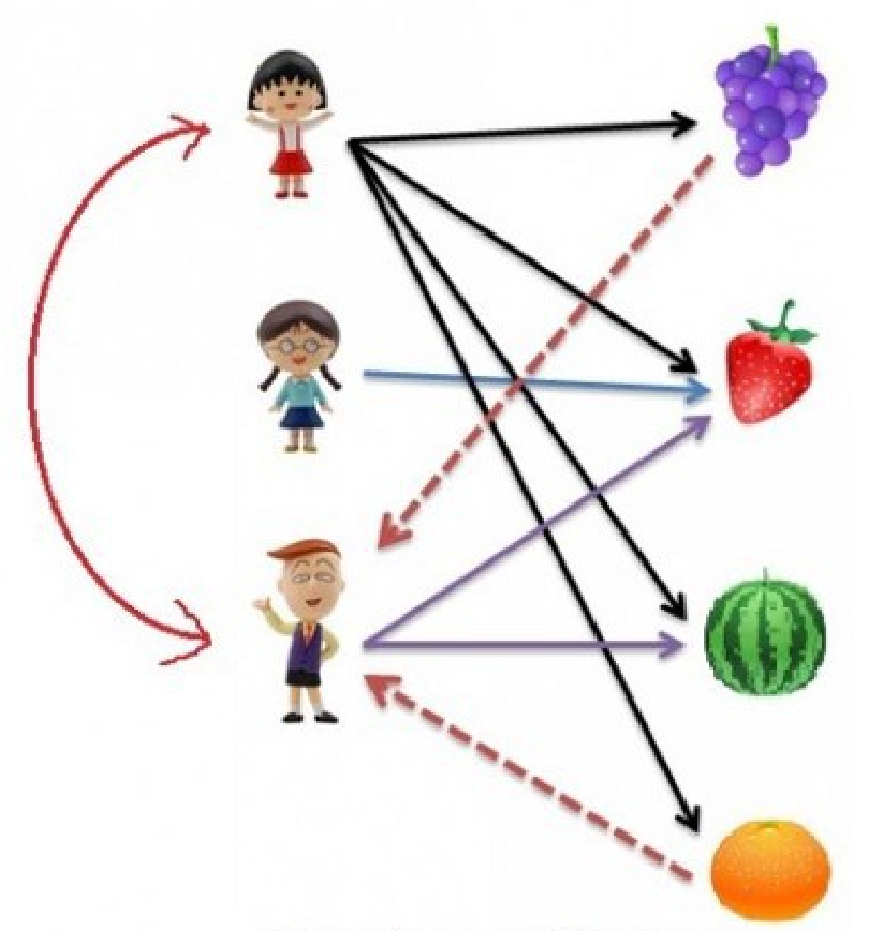
\includegraphics[scale=0.2]{figures/userbased.png}
		\end{figure}
    \end{minipage}
    \newpage
    A specific application of this is the user-based Nearest Neighbor algorithm. This algorithm needs two tasks:
    \begin{enumerate}
        \item Find the K-nearest neighbors (KNN) to the user \textit{a}, using \textit{a} similarity function \textit{w} to measure the distance between each pair of users
        \item Predict the rating that user a will give to all items the k neighbors have consumed but a has not. We Look for the item \textit{j} with the best predicted rating.
    \end{enumerate}
    In other words, we are creating a User-Item Matrix, predicting the ratings on items the active user has not see, based on the other similar users. 
    This technique is memory-based.
\end{frame}
\begin{frame}{User-based filtering}
\framesubtitle{K-nearet neighbors}
    \raggedright
	\begin{minipage}{0.5\linewidth}
        K nearest neighbors is a simple algorithm that stores all available cases and classifies new cases based on a similarity measure (e.g., distance functions).
	\end{minipage}
    \begin{minipage}{0.5\linewidth}
        \begin{figure}
            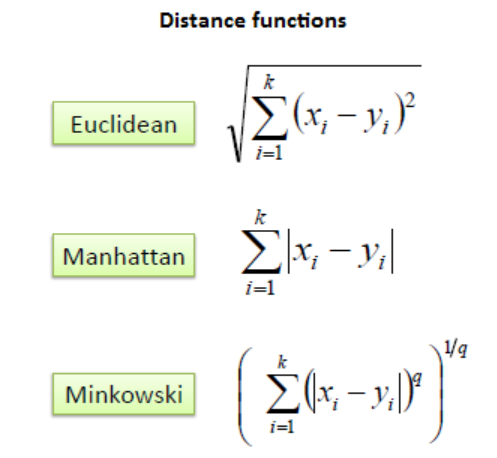
\includegraphics[scale=0.45]{figures/knn.PNG}
		\end{figure}
    \end{minipage}
\end{frame}


\subsection{Item-based}
\begin{frame}[allowframebreaks, fragile]{Protocol}
	\frametitle{Collaborative filtering}
	\framesubtitle{Item-based}
	Back to Stanley. Instead of focusing on his friends, we could focus on what items from all the options are more similar to what we know he enjoys. This new focus is known as Item-Based Collaborative Filtering (IB-CF).
    We could divide IB-CF in two sub tasks:
    \vspace{0.3cm}
    \begin{enumerate}
        \item Calculate similarity among the items:
        \begin{itemize}
            \item Cosine-Based Similarity
            \item Correlation-Based Similarity
            \item Adjusted Cosine Similarity
            \item Jaccard distance
        \end{itemize}
        \newpage
        \item Calculation of Prediction:
        \begin{itemize}
            \item Weighted Sum
            \item Regression
        \end{itemize}.
    \end{enumerate}
    The difference between UB-CF and this method is that, in this case, we directly pre-calculate the similarity between the co-rated items, skipping K-neighborhood search.
\end{frame}
\subsection{Pros and Cons}
\begin{frame}[allowframebreaks, fragile]{Pros ans Cons}
    \textbf{Pros:}
    \begin{itemize}
        \item  Easy to implement.
        \item Context independent.
        \item Compared to other techniques, such as content-based, it is more accurate.
    \end{itemize}
    \textbf{Cons:}
    \begin{itemize}
        \item \textbf{Sparsity:} The percentage of people who rate items is really low.
        \item \textbf{Scalability:} The more K neighbors we consider, the better my classification should be. Nevertheless, the more users there are in the system, the greater the cost of finding the nearest K neighbors will be.
        \item \textbf{Cold-start:} New users will have no to little information about them to be compared with other users.
        \item \textbf{New item:} Just like the last point, new items will lack of ratings to create a solid ranking (More of this on ‘How to sort and rank items’).
    \end{itemize}
\end{frame}